\section{Quantification}\label{sec:quant}

This section puts numbers on the mechanisms. The aim is not to fit every
moment of the arXiv record. It is to check that one parameterisation of the
model reproduces the main facts with plausible primitives, and to read off its
implications for rents, the speed limit, the incidence of research tools,
topic life cycles and growth.

\subsection{Strategy}

We use the functional forms of \cref{sec:model}: harmonic learning
\eqref{eq:Qexample}, exponential detection and the exact catch-up time
\eqref{eq:T}. Time is measured in years. \Cref{tab:calibration} lists the
parameters. Some are set externally. The unit of density is fixed by $b=100$
papers read per year at full-time reading, and production speed by $a=4$
projects per year at full-time production. Careers leave a topic at $\rho=0.10$
(ten-year tenure), the stock's relevance decays at $\delta=0.25$ (a half-life of
about three years), topics become obsolete at $\xi=0.04$, and a newborn topic
produces $P_0=2$ papers a year. The credit block comes from
Fact~\ref{fact:credit} through \cref{lem:credit}. With exponential follow-on
credit and a pivot that costs 30\% of a project, the $+29\%$ premium of aware
follow-ons and the $-19\%$ penalty of unaware duplicates imply that 31\% of
detected overlaps proceed and that detection averts $\Delta/\lambda=37\%$ of
erosion. We set concurrent overlap to zero: our moments do not separate it from
erosion by unread earlier work, and attributing all erosion to unread work
gives reading its largest protective value. Explorers found a viable topic at
rate $s=0.14$, so that half of them found one before their spell ends
($\omega=1/2$). The frontier block splits the calibrated frontier value into
exploration and founding; it does not affect the cross-section, and we report
results for $\omega$ between 0 and 3/4.

The remaining parameters are calibrated jointly: learning ($\beta,\gamma$),
erosion ($\theta\lambda$), search precision ($\sigma$), the frontier value $F$,
catch-up speed $b_c$, and the distributions of diffusion rates and fertility.
The targets are the corrected returns profile of Fact~\ref{fact:hump}: the
gradient per standard deviation of density, the returns of the sparsest,
fourth and densest fifths relative to the middle one ($-11\%$, $+2\%$, $-2\%$),
and the 12\% of researcher-years beyond the peak. We add the recall-corrected
aware share of 60\% at mature density (Fact~\ref{fact:aware}), which
disciplines $\sigma$, and the share of incumbents' time spent reading. Faculty
report about 144 hours a year reading scholarly articles
\citep{tenopirking2008}, about 7\% of a working year. This target disciplines
the time-share value of reading tools (\cref{lem:timeshares}), which the
previous version of the model left free. A soft target puts the incumbents'
log premium $(\rho+\xi)T$ at about 0.15, about a year of catch-up per
seven-year spell in a topic. Since the measured gradient also reflects
audience, this is generous to the catch-up channel. We simulate the stationary
cross-section of topic life cycles and run the arXiv regressions on it. As in
the data, density is measured with error. Only 58\% of a paper's nearest
neighbours fall in its own fine area. We add classical noise with a standard
deviation of 0.3 in log density, which implies a reliability of about 0.8.
Researchers who move between topics supply the identifying variation in an
author-fixed-effects design, and the model has no ability differences. The
baseline analogue is therefore the cross-section of researcher-years. The
within-topic analogue, which uses only life-cycle variation, is a robustness
check. The search is a quasi-random scan of 2,048 points followed by
Nelder--Mead from the best points and from the previous calibration, with the
winner selected on a fine simulation grid (\cref{app:numerics}). The frontier's
depletion $\eta_F$ is then set from \eqref{eq:eta} with $\mathcal E=0.15$
(Fact~\ref{fact:volume}).

\begin{table}[t]
\centering\small
\caption{Parameters}\label{tab:calibration}
\begin{tabular}{@{}llll@{}}
\toprule
Parameter & Meaning & Value & Source \\
\midrule
\multicolumn{4}{@{}l}{\emph{Set externally}} \\
$b$ & papers read per year at full-time reading & 100 & normalisation (unit of $P$) \\
$\lambda$ & credit lost by an unaware duplicate & 0.19 & Fact 3 ($-19\%$) \\
$\kappa_p$ & credit lost by pivoting & 0.30 & assumption \\
$\Delta/\lambda$, $q$ & detection value; share proceeding & 0.37, 0.31 & Fact 3 ($+29\%$), \cref{lem:credit} \\
$\delta$ & decay of the stock's relevance & 0.25 & half-life $\approx$ 2.8 years \\
$\rho$ & rate of leaving a topic & 0.10 & ten-year topic tenure \\
$\xi$ & topic obsolescence & 0.04 & 25-year topic life \\
$P_0$ & flow of a newborn topic & 2 & a few papers per year \\
\multicolumn{4}{@{}l}{\emph{Calibrated (\cref{tab:fit})}} \\
$\beta$, $\gamma$ & learning efficiency, curvature & 39.01, 0.156 & hump in returns \\
$\theta\lambda$ & erosion per earlier paper & 0.0041 & fall at the top \\
$F$ & frontier payoff & 1.768 & sparsest fifth \\
$b_c$ & catch-up reading speed & 25 & premium, share beyond peak \\
$\sigma$ & search precision & 1.58 & recall-corrected aware share \\
$g_{\rm med}$, $s_g$ & diffusion rate: median, log-sd & 0.182, 0.29 & share beyond peak, fifths \\
$s_\zeta$ & log-sd of topic fertility & 0.052 & gradient across topics \\
$\eta$ & frontier elasticity & 0.0067 & $\mathcal{E}=0.15$ (Fact 1), \eqref{eq:eta} \\
\bottomrule
\end{tabular}

\end{table}

\begin{table}[t]
\centering\small
\caption{Fit to the arXiv facts}\label{tab:fit}
\begin{tabular}{@{}lccc@{}}
\toprule
Moment & arXiv & Baseline & Within-topic \\
\midrule
Gradient per SD of density & 0.067 & 0.049 & 0.055 \\
Sparsest fifth vs.\ middle & -0.080 & -0.071 & -0.096 \\
Fourth fifth vs.\ middle & 0.050 & 0.035 & 0.023 \\
Densest fifth vs.\ middle & 0.010 & 0.067 & 0.028 \\
Researcher-years beyond the peak & 0.120 & 0.129 & 0.125 \\
Incumbents' log premium $\kappa P^m$ & 0.150 & 0.189 & 0.172 \\
Peak of $v$ (SD above mean)$^\dagger$ & 1.00 & 0.92 & 1.10 \\
Quadratic: linear term$^\dagger$ & 0.094 & 0.048 & 0.052 \\
Quadratic: squared term$^\dagger$ & -0.047 & -0.001 & -0.009 \\
Aware share of flagged overlap$^\dagger$ & 0.38 & 0.38 & 0.89 \\
\bottomrule
\end{tabular}

\par\smallskip\footnotesize
$^\dagger$ Not targeted. Baseline: cross-section of researcher-years (movers
across topics). Within-topic: topic fixed effects, recalibrated. Density is the
researcher-weighted standardised log flow, measured with noise as in the data.
The reading share is from \citet{tenopirking2008}.
\end{table}

\subsection{Fit}

\Cref{tab:fit} and \cref{fig:test4} compare model and data. The baseline
calibration reproduces the aware share at mature density (\calAware\ against
60\%), the reading share of incumbents' time (\calReadCS\ against 7\%), most of
the share of researcher-years beyond the peak of the payoff curve
(\calBeyond\ against 12\%) and most of the rise from the sparsest fifth
(\calQone\ against $-11\%$). Without targeting it, the peak lies \calZhat\
standard deviations above mean density, against about one in the data. The
gradient falls short (\calLin\ against 6.7\%), and so does the incumbents'
premium, which is generous to the catch-up channel because the measured
gradient also reflects audience. Exact catch-up makes the problem harder than
it was with the linear approximation: the newcomer's payoff curve now falls
about twice as steeply at the mature density, and fast topics stop well below
the densities they reached before, so the life cycle generates less
overshooting for a given distribution of diffusion rates.

The model still does not reproduce the top of the profile. In the corrected
data the densest fifth earns \emph{less} than the middle ($-2\%$). In the model
the fourth and densest fifths earn \calQfour\ and \calQfive. The source of the
miss is composition. The densest researcher-years in the model include the most
fertile mature topics, whose incumbents earn high returns, alongside the
overshooting topics that pull returns down. Erosion in mature topics is small,
about \calErosion\ of credit, so the payoff curve falls only gently beyond its
peak. The fall at the top points to crowding costs in dense topics beyond
duplication and catch-up, to concurrent overlap, which we set to zero, or to
audience effects that flatter the middle of the distribution. We regard it as
the model's main quantitative failure. \calShareMature\ of researcher-years are
in mature topics, \calShareCons\ in topics consolidating after a growth spurt or
declining after a stall, and \calShareGrowth\ in growing topics. The
within-topic calibration fits its moments more closely (\cref{tab:fit}). Its
median diffusion rate is low, \calWGmed\ a year, so young topics grow slowly and
the life-cycle variation it relies on is spread over many years; relaxing the
bounds of the search does not change it.

\begin{figure}[t]
\centering
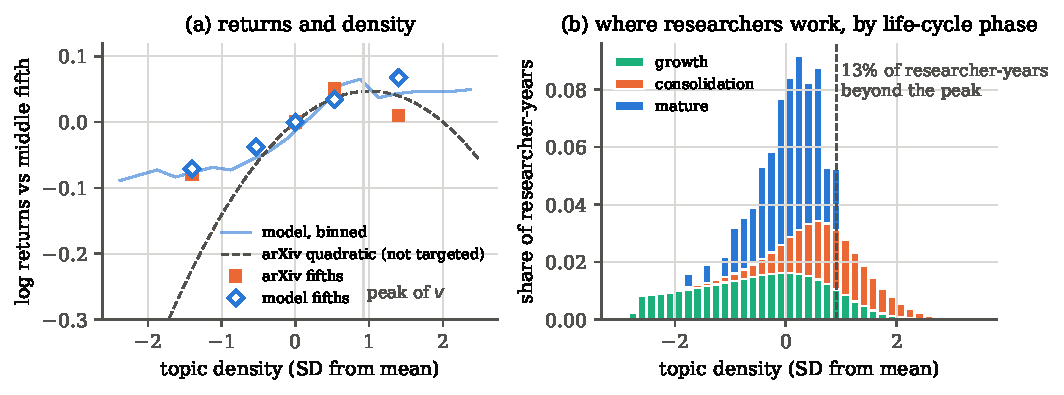
\includegraphics[width=\textwidth]{figures/fig4_test4.pdf}
\caption{Returns and density in the model. Left: log returns by observed (noisily
measured) topic density, relative to the middle fifth, in the calibrated
cross-section, with the arXiv fifths and the arXiv quadratic (not targeted).
Right: the distribution of researcher-years by true density and life-cycle phase.
Researcher-years beyond the peak of $v$ are concentrated in topics consolidating
after fast growth.}
\label{fig:test4}
\end{figure}

\subsection{What the calibrated model says}

\Cref{tab:welfare} collects the implications.

\begin{table}[t]
\centering\small
\caption{Rents, the speed limit, welfare and growth in the calibrated model}\label{tab:welfare}
\begin{tabular}{@{}lr@{}}
\toprule
Object & Value \\
\midrule
Peak of the payoff curve $\hat P$ (papers per year) & 23.4 \\
Gain from cumulative knowledge at the peak, $\hat v/v(P_0)-1$ & 17.0\% \\
Mature density $P^m$ & 12.0 \\
Catch-up time $T=S/b_c$ (years) & 1.68 \\
Incumbents' premium over the frontier, $e^{\kappa P^m}-1$ & 18.3\% \\
Rent at the peak, $\hat v/F-1$ & 20.1\% \\
Frictionless benchmark: rent dissipated, $1-F/\hat v$ & 16.7\% \\
Catch-up economy: planner's gain, $\hat w/F-1$ & 4.4\% \\
Optimal frontier subsidy, $s^o/F$ & 4.4\% \\
Overshooting threshold $g^*$ (per year) & 0.197 \\
Slope of the entrant payoff curve $|\varepsilon_w(P^m)|$ & 0.125 \\
Frontier elasticity $\eta$ (from $\mathcal{E}=0.2$) & 0.0328 \\
Stepping-on-toes parameter $\lambda_J=1-\mathcal{E}|\varepsilon_w|$ & 0.975 \\
\bottomrule
\end{tabular}

\end{table}

\paragraph{Rents and the speed limit.} The payoff curve peaks at
$\Phat=\calPhat$ papers a year, the newcomer's payoff curve at
$\hat P_w=\calPw$, and mature topics sit between them, at $P^m=\calPm$. The speed
limit is $b_c=\calBc$ papers a year: mature topics sit at \calSpeedRatio\ of it,
and the most fertile at \calSpeedRatioTop. Catching up takes \calT\ years at the
mature density and \calTpeak\ at the peak. Incumbents earn a premium of
\calPremium\ over the frontier, and the cross-topic returns gradient, the
catch-up elasticity $\eps_\Gamma=\calEpsG$, is steeper than the premium, as
\cref{prop:mature}(iv) requires. Even with rising incumbent returns
($\eps_v(P^m)=\calEpsV>0$), the newcomer's payoff curve is falling at the mature
density ($|\eps_w|=\calEpsW$), so mature topics are too crowded once the
catch-up burden is counted (\cref{cor:overcrowd}). Moving every topic to the
peak of $w$ raises output per researcher by \calPlannerGain\ (\calWPlannerGain\
in the within-topic calibration). The frictionless benchmark, in which catch-up
is free and topics fill to the density where $v=F$, would dissipate \calDissip\
of output per researcher. That number describes a counterfactual economy, not
the calibrated one.

\paragraph{The incidence of research tools.} \Cref{tab:ai,tab:incidence} and
\cref{fig:incidence} report the effects of 30\% improvements in each channel.
Reading takes \calRm\ of an incumbent's time at the mature density, so faster
reading is worth $r^*/(1-r^*)=\calTimeValueRead$ per log point at a fixed topic:
a 30\% faster reader gains \calReadFixed\ log points, a 30\% faster producer
\calWriteFixed. Per hour saved, the two are worth the same. Entry then ranks
them. The producer keeps almost everything, \calWriteOut\ log points. If
explorers never stay in the topics they open, the reader keeps
\calReadOutNoF\ log points, \calReadPassNoF\ of her gain, close to the floor
$\mathcal ED$ of \eqref{eq:passthrough}. If founders stay with probability one
half, she keeps \calReadOut, or \calReadPass. Per hour saved, a production tool
is therefore worth between \calPerHour\ and \calPerHourNoF\ times a reading
tool. Catch-up tools keep \calCatchPassNoF\ without founders and \calCatchPass\
with them; founders never catch up, so their gain reaches the frontier only
through the density of the topics founders end up in.

On the simulated life cycle the founders' channel is weaker for catch-up
tools and somewhat weaker for reading tools. Founders spend much of their
tenure in topics still growing at a pace set by diffusion, so the frontier
value rises by \calLCReadF\ of a reading gain and by only \calLCCatchF\ of a
catch-up gain. Output per researcher-year, which also counts the rents of
newcomers who enter growing topics before entry pays only the frontier value,
rises by more: \calLCReadY\ of a reading gain (\calLCReadYnoF\ without founders),
\calLCCatchY\ of a catch-up gain and \calLCProdY\ of a production gain. These
rents raise life-cycle output per researcher \calLCRent\ above the frontier
value. The footprints in \cref{tab:ai} follow \cref{prop:ai}. Faster reading
raises density by \calReadDens\ log points; faster catch-up raises it by
\calCatchDens\ and lowers the overshooting threshold by \calCatchGstar\
percentage points, so more topics grow too fast; better search raises the aware
share by \calSearchAware\ percentage points.

\begin{table}[t]
\centering
\caption{How much of each tool survives entry, and readership}\label{tab:incidence}
\small
\begin{tabular}{@{}lrrrrrr@{}}
\toprule
 & \multicolumn{2}{c}{Faster reading} & \multicolumn{2}{c}{Faster catch-up} & \multicolumn{2}{c}{Faster production} \\
\cmidrule(lr){2-3}\cmidrule(lr){4-5}\cmidrule(l){6-7}
 & formula & life cycle & formula & life cycle & formula & life cycle \\
\midrule
\multicolumn{7}{@{}l}{\emph{A. Share of the gain at fixed topics that survives entry (\%)}} \\
$\omega=0.00$ & 17 & 40 & 17 & 11 & 99 & 99 \\
$\omega=0.25$ & 50 & 44 & 31 & 17 & 99 & 99 \\
$\omega=0.50$ & 74 & 63 & 41 & 17 & 99 & 99 \\
$\omega=0.75$ & 91 & 79 & 48 & 16 & 99 & 99 \\
\midrule
\multicolumn{7}{@{}l}{\emph{B. Long-run gain valued by readership, $\omega=0.5$ (log points $\times100$)}} \\
$\alpha=0.0$ & \multicolumn{2}{c}{$+1.5$} & \multicolumn{2}{c}{$+1.0$} & \multicolumn{2}{c}{$+26.0$} \\
$\alpha=0.5$ & \multicolumn{2}{c}{$+11.3$} & \multicolumn{2}{c}{$+6.3$} & \multicolumn{2}{c}{$+13.6$} \\
$\alpha=1.0$ & \multicolumn{2}{c}{$+21.2$} & \multicolumn{2}{c}{$+11.5$} & \multicolumn{2}{c}{$+1.3$} \\
\bottomrule
\end{tabular}
\par\smallskip\footnotesize Panel A: \emph{formula} is the frontier-incidence pass-through at the mature density (\cref{thm:incidence}) with founders' topics valued at maturity and $\eta_F$ set from the volume elasticity; \emph{life cycle} re-solves the founders' fixed point $F=(1-\omega)e+\omega\bar U_F(F)$ on the simulated life cycle (no depletion) and measures output per researcher-year with exploration, catch-up and diffusion rents counted. Panel B: output valued as $A^\alpha Y$, where $A=(b/a)r^*/(1-r^*)$ is reads per paper; $\alpha=0$ is credited output, $\alpha=1$ readership.

\end{table}

\begin{figure}[t]
\centering
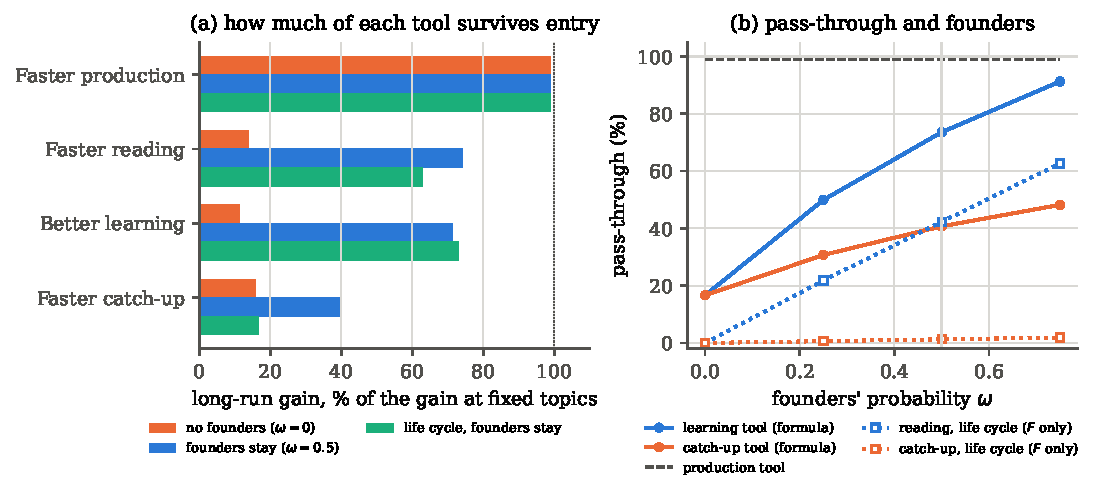
\includegraphics[width=\textwidth]{figures/fig5_incidence.pdf}
\caption{The incidence of research tools in the calibrated model (30\% shocks).
Left: long-run gain in output per researcher as a share of the gain at fixed
topics, without founders, with founders who stay (stationary), and on the
simulated life cycle. Right: the share that survives entry as a function of
the founders' probability $\omega$, from the incidence formula and, for the
frontier value alone, on the life cycle.}
\label{fig:incidence}
\end{figure}

\paragraph{Readership.} Valued by readership ($\alpha=1$ in
\cref{prop:audience}), a 30\% faster pen adds \calAudWrite\ log points and 30\%
faster reading \calAudRead: a faster pen leaves total reading unchanged and
cuts reads per paper by \calReadsDrop. With readership given half the weight of
credit ($\alpha=1/2$) the two tools are worth about the same, \calAudWriteHalf\
and \calAudReadHalf\ log points. Which tool scales science depends on the unit,
and the unit is a choice about what science values.

\paragraph{Topic life cycles.} A newborn topic beats the frontier by
\calNewborn, so its first followers join, but a stationary topic of the same
density would not be worth joining. Topics that grow more slowly than
\calGtakeoff\ a year stall in the valley and are abandoned, and topics that grow
faster than \calGstarExact\ overshoot the peak (\cref{prop:toofast}); with
foresight the overshooting threshold is \calGstarRE. These are fast but not
unusual rates for hot topics on arXiv.

\paragraph{Growth.} Inverting \eqref{eq:eta} with $\mathcal E=0.15$ gives a frontier
depletion of $\eta_F=\calEta$ (\calEtaNoF\ without founders), and the
stepping-on-toes parameter is $\lambda_J^{\rm eq}=1-\mathcal E|\eps_w|=\calLambda$ when
topics adjust and $\lambda_J^M=1+\eps_w/D=\calLambdaFixed$ when open topics are
held fixed (\cref{prop:sot}). Over the arXiv range $\mathcal E\in[0,0.27]$,
$\lambda_J^{\rm eq}$ lies between \calLambdaLo\ and one. The short-run bias from
topic-age composition (\cref{rem:shortrun}) is $-\calCompBias$ over a
seven-year window, so even the upper end of the long-run range keeps
$\lambda_J^{\rm eq}$ close to one. Topic crowding and access depletion explain
little of the diminishing returns to research found by \citet{bloometal2020}.
Their estimates require $\lambda_J$ well below one, which in our framework must
come from fertility depletion (\cref{app:fertility}) or from selection.
